%% Apêndices

\begin{apendicesenv}

% Imprime uma página indicando o início dos apêndices
\partapendices

% Apêndice A -- Documento de Requisitos do Sistema (versão 1.1, assinada)
\chapter{Documento de Requisitos do Sistema}\label{apendice-requisitos}

O Documento de Requisitos do Sistema, em sua versão 1.1, elaborado pela equipe e assinado digitalmente pela parceira do projeto e pelos integrantes do grupo, é reproduzido integralmente nas páginas a seguir.

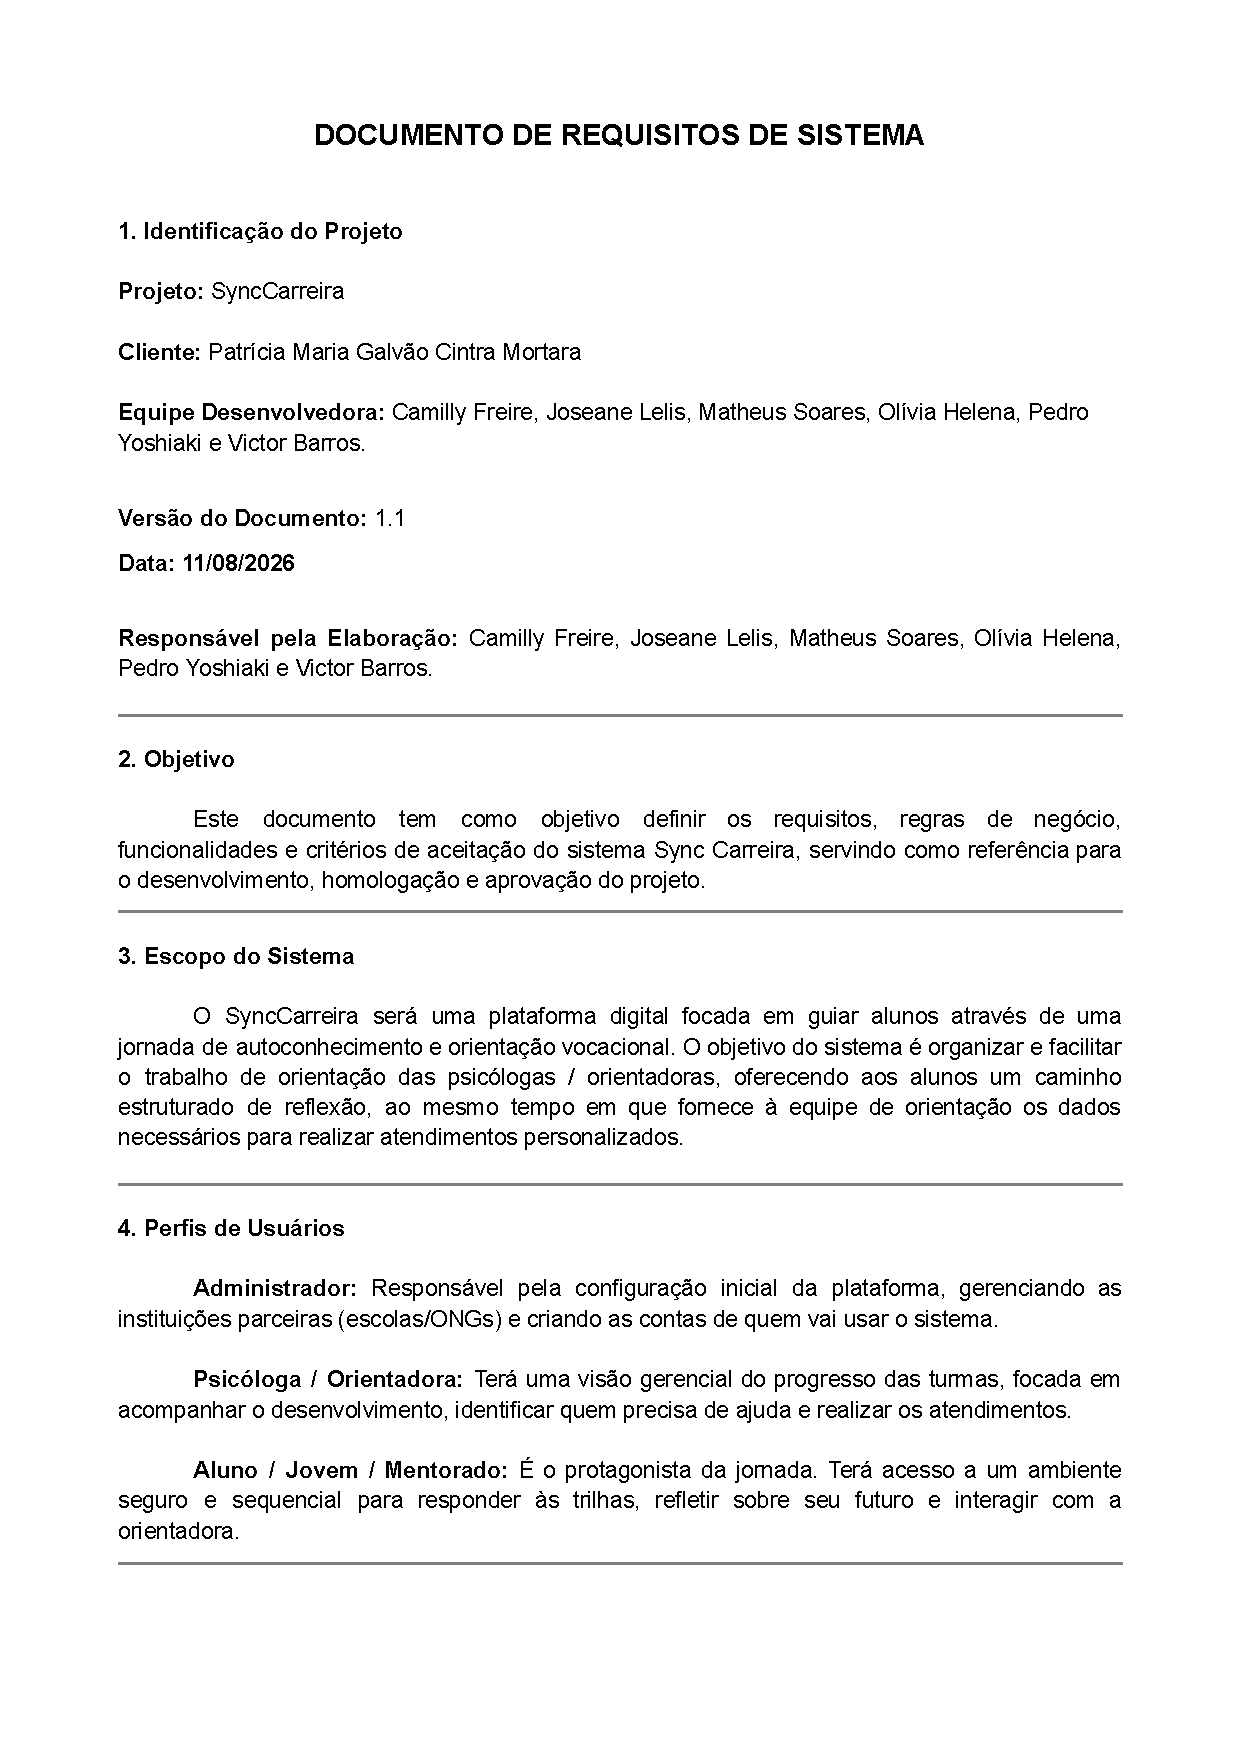
\includepdf[pages=-,scale=0.85,frame,pagecommand={\thispagestyle{abntnumero}}]{pos-textual/documento-requisitos.pdf}

% Apêndice B -- Resultados da análise estática no SonarCloud
\chapter{Resultados da Análise Estática no SonarCloud}\label{apendice-sonar}

Este apêndice reproduz o painel de visão geral do projeto no SonarCloud, capturado em 4 de novembro de 2026, com os resultados da análise estática do código. A \autoref{fig_sonar_geral} apresenta a situação do \textit{quality gate}, a quantidade de apontamentos, a duplicação de código, a cobertura de testes e os indicadores de segurança. A \autoref{fig_sonar_qualidade} apresenta os indicadores de confiabilidade e de manutenibilidade.

\begin{figure}[p]
    \centering
    \caption{Painel do SonarCloud: situação geral e segurança.}
    \label{fig_sonar_geral}
    \fbox{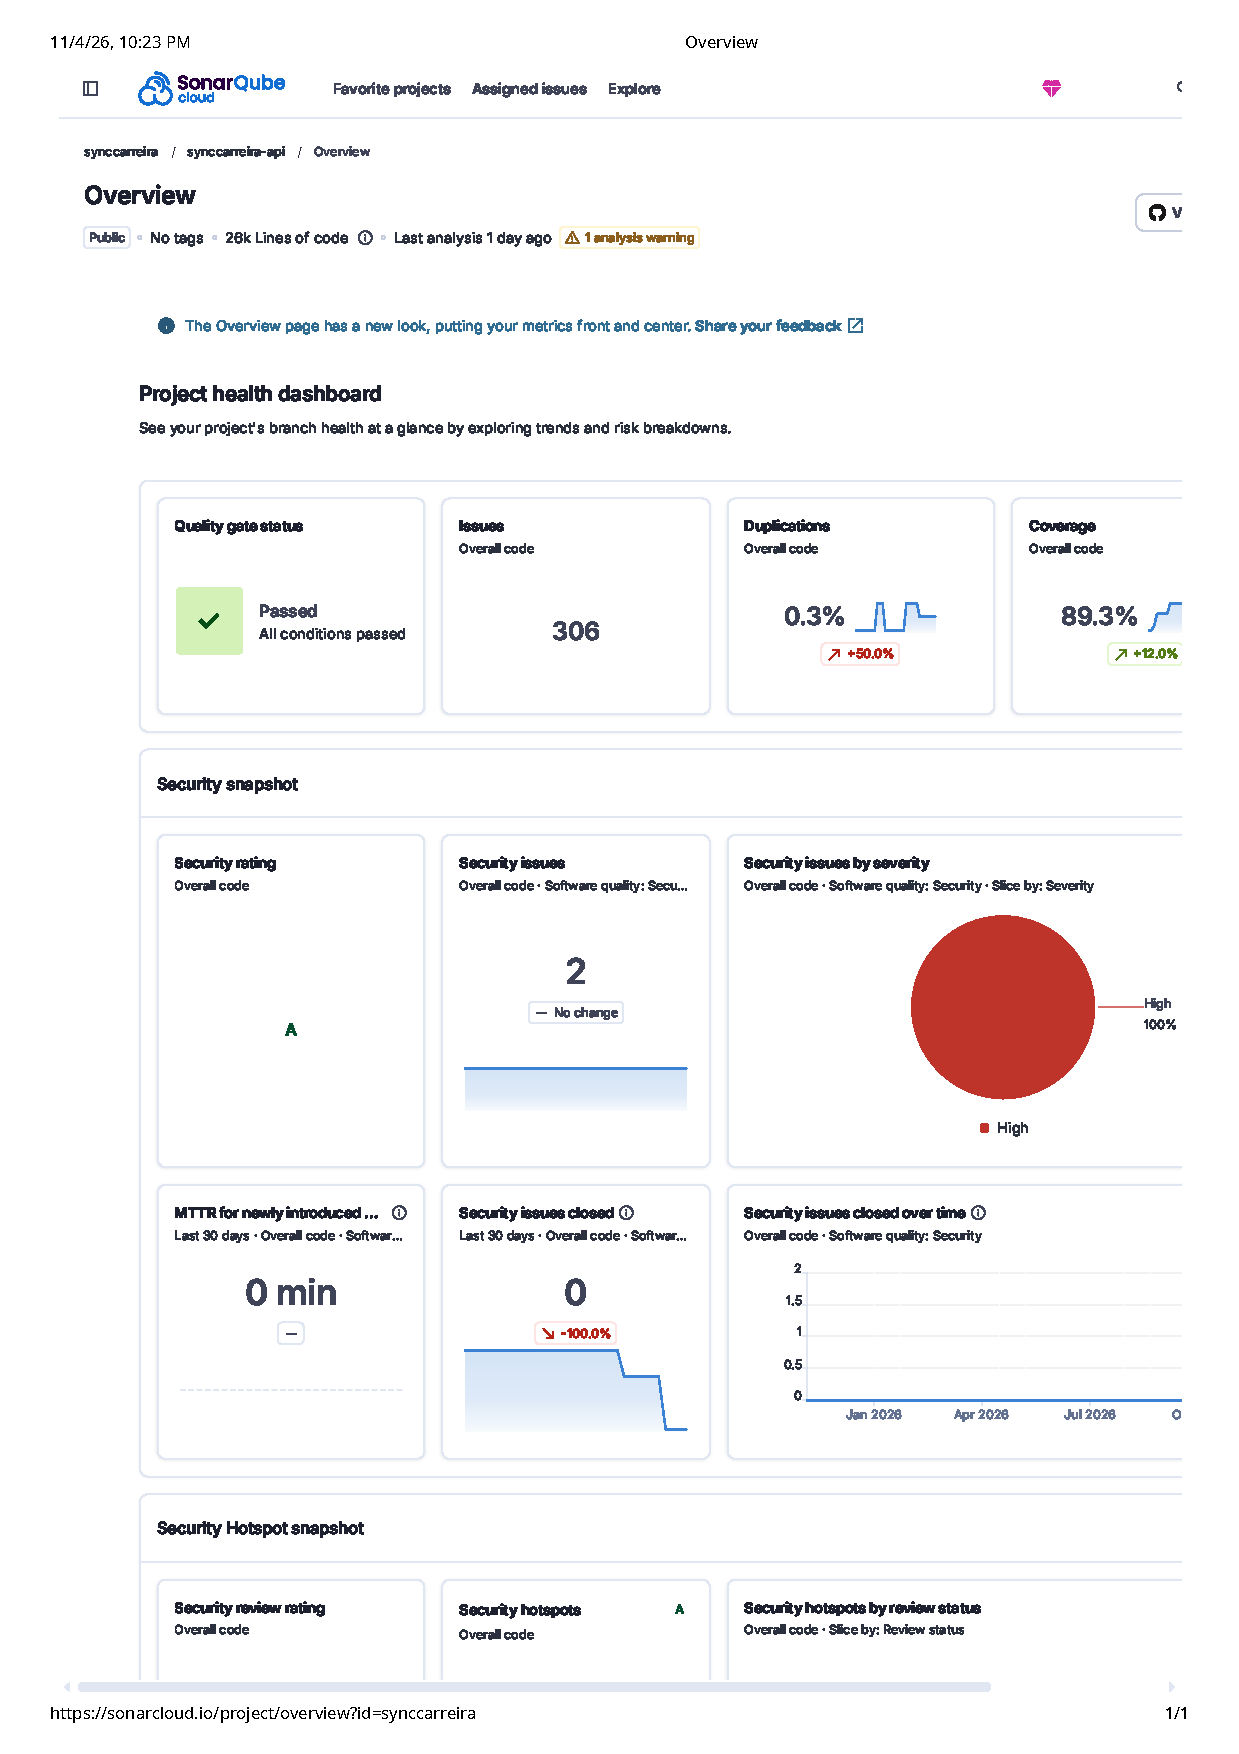
\includegraphics[page=1,height=0.8\textheight]{pos-textual/sonarcloud-painel-1.pdf}}
    \legend{Fonte: SonarCloud (2026).}
\end{figure}

\begin{figure}[p]
    \centering
    \caption{Painel do SonarCloud: confiabilidade e manutenibilidade.}
    \label{fig_sonar_qualidade}
    \fbox{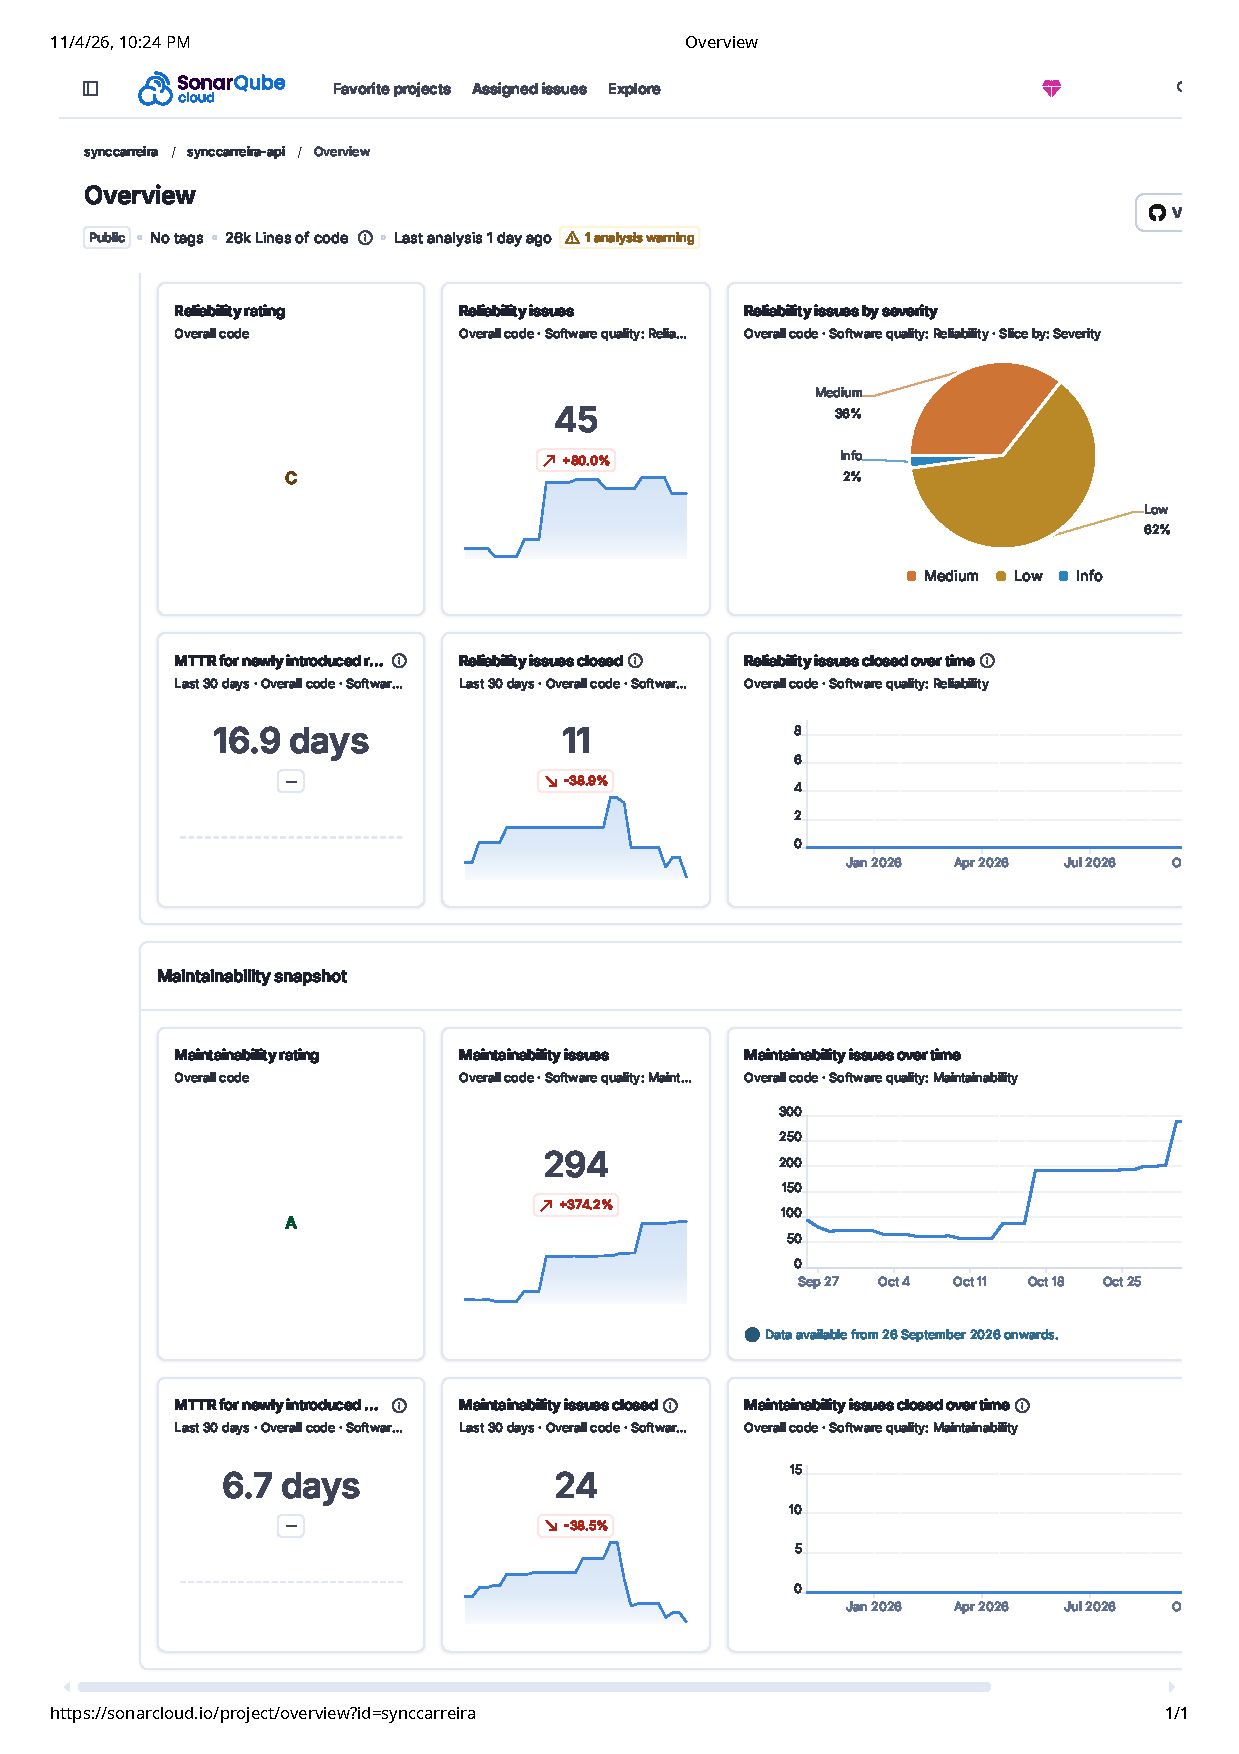
\includegraphics[page=1,height=0.8\textheight]{pos-textual/sonarcloud-painel-2.pdf}}
    \legend{Fonte: SonarCloud (2026).}
\end{figure}

% Apêndice C -- Plano de Garantia da Qualidade e Testes de Software
\chapter{Plano de Garantia da Qualidade e Testes de Software}\label{apendice-plano-testes}

Este apêndice reproduz o plano de garantia da qualidade e testes de \textit{software} elaborado pela equipe para o \textit{SyncCarreira}, em sua versão de planejamento.

\section*{1 Identificação do Projeto e Governança}

{\ABNTEXfontereduzida
\renewcommand{\arraystretch}{1.25}
\begin{xltabular}{\textwidth}{|>{\raggedright\arraybackslash}p{4.2cm}|>{\raggedright\arraybackslash}X|}
\multicolumn{2}{@{}c@{}}{\quadrolongocaption{Identificação do projeto e governança.}\label{quadro-plano-identificacao}} \\[0.3em]
\hline
\textbf{Item de governança} & \textbf{Descrição e dados de registro} \\
\hline
\endfirsthead
\multicolumn{2}{@{}r@{}}{\textit{(continuação)}} \\
\hline
\textbf{Item de governança} & \textbf{Descrição e dados de registro} \\
\hline
\endhead
\multicolumn{2}{@{}r@{}}{\textit{(continua)}} \\
\endfoot
\endlastfoot
Nome do projeto & \textit{SyncCarreira} \\
\hline
Propósito do sistema & Plataforma digital integrada para psicólogas, escolas e alunos, estruturada para guiar o autoconhecimento profissional e mitigar a evasão universitária. \\
\hline
Cliente / responsável técnica & Patrícia Maria Galvão Cintra Mortara \\
\hline
Equipe desenvolvedora (IFSP) & Camilly Freire, Joseane Lelis, Matheus Soares, Olívia Helena, Pedro Yoshiaki e Victor Barros \\
\hline
Curso e instituição & Tecnologia em Análise e Desenvolvimento de Sistemas --- Instituto Federal de Educação, Ciência e Tecnologia de São Paulo \\
\hline
Versão do documento & 1.0 --- Planejamento inicial \\
\hline
\end{xltabular}
\legend{Fonte: Autoria própria (2026).}
}

\section*{2 Objetivos e Diretrizes Estratégicas}

Este plano tem por finalidade estabelecer a estratégia formal de garantia de qualidade para o sistema \textit{SyncCarreira}, alinhando as melhores práticas de Engenharia de \textit{Software} às exigências de rigor acadêmico da banca examinadora.

\section*{3 Delimitação do Escopo de Testes}

O escopo do plano delimita quais tipos de testes e requisitos do sistema serão submetidos à verificação formal, bem como as exclusões deliberadas do projeto.

{\ABNTEXfontereduzida
\renewcommand{\arraystretch}{1.25}
\begin{xltabular}{\textwidth}{|>{\raggedright\arraybackslash}p{4.0cm}|>{\raggedright\arraybackslash}p{2.4cm}|>{\raggedright\arraybackslash}X|}
\multicolumn{3}{@{}c@{}}{\quadrolongocaption{Delimitação do escopo de testes.}\label{quadro-plano-escopo}} \\[0.3em]
\hline
\textbf{Categoria de verificação} & \textbf{Status} & \textbf{Justificativa e critério acadêmico} \\
\hline
\endfirsthead
\multicolumn{3}{@{}r@{}}{\textit{(continuação)}} \\
\hline
\textbf{Categoria de verificação} & \textbf{Status} & \textbf{Justificativa e critério acadêmico} \\
\hline
\endhead
\multicolumn{3}{@{}r@{}}{\textit{(continua)}} \\
\endfoot
\endlastfoot
Análise estática de código & Obrigatório & Requisito obrigatório para identificação precoce de vulnerabilidades. \\
\hline
Testes unitários ($\geq$ 80\%) & Obrigatório & Requisito mandatório, com meta mínima de 80\% de cobertura, para proteger as regras de negócio críticas do sistema. \\
\hline
Testes \textit{cross-browser} & Obrigatório & Testes em pelo menos dois motores de navegação distintos (Google Chrome e Mozilla Firefox), validando a responsividade \textit{mobile-first} (RNF-04). \\
\hline
Testes E2E / BDD (aceitação) & No escopo & Validação ponta a ponta dos fluxos operacionais de Administrador, Psicóloga e Aluno por meio de cenários Gherkin. \\
\hline
Testes de carga e estresse & No escopo & Validação com massa de dados para verificar a capacidade de processamento do sistema. \\
\hline
Validação psicométrica clínica & Fora de escopo & O escopo do \textit{software} restringe-se à infraestrutura digital; os instrumentos psicológicos são de domínio público ou fornecidos pela parceira técnica. \\
\hline
\end{xltabular}
\legend{Fonte: Autoria própria (2026).}
}

\section*{4 Estratégia Detalhada por Nível de Teste}

\subsection*{4.1 Análise estática de código (inspeção pré-execução)}

A análise estática será executada de forma automatizada no fluxo de integração contínua, avaliando o código-fonte sem a necessidade de sua execução. Os critérios estabelecidos compreendem:

\begin{itemize}
  \item \textbf{conformidade de estilo e padronização}: garantir legibilidade uniforme entre todos os membros da equipe técnica;
  \item \textbf{detecção de \textit{code smells} e dívida técnica}: sinalização imediata de duplicações de lógica, funções excessivamente extensas ou acoplamento excessivo;
  \item \textbf{segurança de dados}: identificação de vulnerabilidades potenciais e de vazamento de informações sensíveis, em alinhamento ao RNF-02 e à LGPD;
  \item \textbf{critério de aceitação}: zero apontamentos classificados com severidade crítica ou bloqueante.
\end{itemize}

\subsection*{4.2 Testes unitários e meta de cobertura ($\geq$ 80\%)}

Os testes unitários têm como foco as unidades funcionais isoladas das camadas de domínio e de regras de negócio, utilizando objetos simulados (\textit{mocks} e \textit{stubs}) para isolar as interações com bancos de dados ou serviços externos. A meta global é atingir no mínimo 80\% de cobertura de linhas e de ramificações lógicas (\textit{branch coverage}). Os módulos com cobertura prioritária obrigatória são:

\begin{itemize}
  \item \textbf{validador cadastral}: algoritmo de validação dos dígitos verificadores do CNPJ, além de formatos válidos de e-mail e de datas;
  \item \textbf{gerenciador de estado da jornada (RN-01 e RN-02)}: regra que impede o desbloqueio da trilha seguinte sem a conclusão integral da anterior e valida a presença obrigatória da síntese livre;
  \item \textbf{motor do leque de carreiras (RF-12 e RN-07)}: algoritmo de ponderação de interesses que garante a entrega de múltiplos caminhos formativos, sem diagnósticos fechados;
  \item \textbf{filtro de indecisão (RF-04 e RN-04)}: lógica de negócio que destaca no painel e prioriza para sessões de orientação os alunos que concluem a jornada sinalizando dúvida.
\end{itemize}

\subsection*{4.3 Testes de integração e isolamento entre instituições}

Validação da camada de persistência e da segurança de dados, garantindo que o requisito não funcional de isolamento de dados por instituição (RNF-08) e o controle de acesso baseado em papéis (RNF-01) sejam respeitados:

\begin{itemize}
  \item tentativas simuladas de acesso a dados de alunos e turmas de uma escola ``A'' por uma psicóloga vinculada à escola ``B'' devem retornar o código HTTP 403 (\textit{Forbidden}) ou lista vazia;
  \item preservação do sigilo das respostas individuais da trilha nas visualizações gerais do painel da orientadora (RN-03).
\end{itemize}

\subsection*{4.4 Testes \textit{cross-browser} (compatibilidade entre navegadores)}

Como o sistema é concebido como uma aplicação \textit{web} responsiva sob a abordagem \textit{mobile-first} (RNF-04), os testes visuais e funcionais serão executados em dois navegadores de referência, com motores de renderização distintos.

{\ABNTEXfontereduzida
\renewcommand{\arraystretch}{1.25}
\begin{xltabular}{\textwidth}{|>{\raggedright\arraybackslash}p{3.4cm}|>{\raggedright\arraybackslash}p{3.6cm}|>{\raggedright\arraybackslash}X|}
\multicolumn{3}{@{}c@{}}{\quadrolongocaption{Navegadores de referência para os testes.}\label{quadro-plano-navegadores}} \\[0.3em]
\hline
\textbf{Navegador} & \textbf{Motor de renderização} & \textbf{Aspectos inspecionados} \\
\hline
\endfirsthead
\multicolumn{3}{@{}r@{}}{\textit{(continuação)}} \\
\hline
\textbf{Navegador} & \textbf{Motor de renderização} & \textbf{Aspectos inspecionados} \\
\hline
\endhead
\multicolumn{3}{@{}r@{}}{\textit{(continua)}} \\
\endfoot
\endlastfoot
Google Chrome & Blink / V8 & Comportamento padrão em \textit{desktop} e emulação de \textit{viewport} de \textit{smartphones}; escalas Likert. \\
\hline
Mozilla Firefox & Gecko / SpiderMonkey & Compatibilidade em ambiente corporativo e educacional, renderização das folhas de estilo (\textit{Flexbox} e \textit{Grid}) e validação de formulários. \\
\hline
\end{xltabular}
\legend{Fonte: Autoria própria (2026).}
}

\subsection*{4.5 Testes de sistema e aceitação em BDD (Gherkin)}

O comportamento esperado do sistema será modelado segundo o padrão BDD, adotando as palavras-chave Dado (pré-condição), Quando (ação única de estímulo) e Então (resultado esperado observável). Isso assegura comunicação transparente com a cliente e serve como base para a automação de testes funcionais ponta a ponta.

\section*{5 Matriz de Mapeamento: Requisitos e Abordagem de Testes}

{\ABNTEXfontereduzida
\renewcommand{\arraystretch}{1.25}
\begin{xltabular}{\textwidth}{|>{\raggedright\arraybackslash}p{2.1cm}|>{\raggedright\arraybackslash}p{3.3cm}|>{\raggedright\arraybackslash}p{3.4cm}|>{\raggedright\arraybackslash}X|}
\multicolumn{4}{@{}c@{}}{\quadrolongocaption{Matriz de mapeamento entre requisitos e abordagem de testes.}\label{quadro-plano-matriz}} \\[0.3em]
\hline
\textbf{Requisito / regra} & \textbf{Descrição do comportamento} & \textbf{Nível de teste} & \textbf{Critério de verificação} \\
\hline
\endfirsthead
\multicolumn{4}{@{}r@{}}{\textit{(continuação)}} \\
\hline
\textbf{Requisito / regra} & \textbf{Descrição do comportamento} & \textbf{Nível de teste} & \textbf{Critério de verificação} \\
\hline
\endhead
\multicolumn{4}{@{}r@{}}{\textit{(continua)}} \\
\endfoot
\endlastfoot
RF-01, RF-02 & Gestão de instituições e usuários & Unitário + BDD (@admin\_gestao) & Criação válida de contas, associação correta às escolas e bloqueio de CNPJ e e-mail duplicados. \\
\hline
RF-03, RF-04, RF-05 & Painel da orientadora e triagem de alunos em dúvida & Unitário + BDD (@painel\_psicologa) & Exibição correta do progresso das trilhas sem exposição das respostas (RN-03) e filtro de alunos em dúvida (RN-04). \\
\hline
RF-06 & Curadoria de \textit{links} externos & BDD (@curadoria\_links) & Exibição precisa dos \textit{links} cadastrados na trilha de Informação (RN-05). \\
\hline
RF-08, RF-09, RF-16 & Sessões, Google Agenda e \textit{feedbacks} & Integração + BDD (@sessoes\_feedback) & Disparo correto dos convites de calendário e visualização exclusiva do \textit{feedback} na área do aluno. \\
\hline
RF-10, RF-11, RN-01, RN-02 & Jornada sequencial de trilhas e síntese reflexiva & Unitário + BDD (@jornada\_trilhas) & Bloqueio do avanço para a trilha subsequente sem conclusão e sem texto livre registrado. \\
\hline
RF-12, RN-07 & Leque aberto de carreiras sugeridas & Unitário + BDD (@resultados\_aluno) & Validação de que a saída apresenta um leque de possibilidades profissionais sem impor diagnóstico fechado. \\
\hline
RNF-01, RNF-08 & Segurança e isolamento entre instituições & Integração / segurança & Impossibilidade de vazamento de informações entre instituições distintas cadastradas no sistema. \\
\hline
RNF-04 & Responsividade e usabilidade \textit{mobile-first} & \textit{Cross-browser} (Chrome e Firefox) & Navegação íntegra, fluida e legível em resoluções de \textit{desktop} e de dispositivos móveis, sem necessidade de manuais. \\
\hline
\end{xltabular}
\legend{Fonte: Autoria própria (2026).}
}

\section*{6 Critérios de Homologação e Definição de Conclusão}

A etapa de testes será formalmente considerada concluída e aprovada para apresentação perante a banca examinadora mediante o atendimento simultâneo aos seguintes critérios:

\begin{enumerate}[label=\arabic*.]
  \item \textbf{comprovação de cobertura unitária}: relatório consolidado demonstrando índice de cobertura de testes igual ou superior a 80\% nas classes de regras de negócio;
  \item \textbf{relatório de análise estática}: ausência de vulnerabilidades de segurança e de apontamentos de severidade crítica no código-fonte;
  \item \textbf{execução integral dos cenários BDD}: 100\% dos cenários de comportamento (caminhos principais e de exceção) executados com situação aprovada;
  \item \textbf{validação em múltiplos navegadores}: testes de conformidade de \textit{layout} e de fluxo executados e aprovados no Google Chrome e no Mozilla Firefox;
  \item \textbf{ausência de defeitos críticos}: nenhum incidente aberto que viole o isolamento de dados entre escolas parceiras ou interrompa a jornada reflexiva do estudante.
\end{enumerate}

\end{apendicesenv}
